\section{Bestimmung der Relaxationslänge}

Es wird vorgegangen wie in der Vorbereitung beschrieben. Auf den Abstand $r$ von der Quelle wird eine Unsicherheit von $\Delta r=\SI{1}{\milli\metre}$ angenommen. Die Skalenbreite betrug $\SI{1}{\milli\metre}$, was einer Unsicherheit von $\SI{0,5}{\milli\metre}$ entsprechen würde. Es ist jedoch auch möglich, dass die Quelle ungenau positioniert wurde.
Die Anzahl der detektierten Neutronen folgt einer Poisson-Verteilung, weshalb die Unsicherheit $\Delta N=\sqrt{N}$ beträgt. Da die Fehler unkorreliert sind, wird die gaußsche Fehlerfortpflanzung verwendet. Es ergibt sich für die Unsicherheit von $y=\ln(Nr^{2})$
\begin{equation}
 \Delta y = \sqrt{\frac{1}{N}+\left(\frac{2\Delta r}{r}\right)^{2}}.
\end{equation}

Die lineare Regression der Form $y=ar+b$ wird mit ``kafe'' durchgeführt und ergibt (s. Abb. \ref{fig:plot1})
\begin{equation}
 a = \SI{-0,077\pm0,003}{\per\centi\metre}.
\end{equation}
Daraus folgt für die Relaxationslänge
\begin{equation}
 \lambda = -\frac{1}{a} = \SI{12,9\pm0,5}{\centi\metre}.
\end{equation}
Der Literaturwert für $\lambda$ ist $\SI{9,58}{\centi\metre}$ \cite{Tittman}. Dies liegt außerhalb der Fehlergrenzen unseres Messwertes. Die Abweichung beträgt ca. $35\%$. Der Grund dafür ist vermutlich, dass die Voraussetzungen für das angenommene Flussgesetz nicht erfüllt sind. Somit hat das gemessene $\lambda$ auch nicht die in der Vorbereitung beschriebene physikalische Bedeutung.

Zusätzlich wurde das Flussgesetz noch für die Messwerte mit Abschirmung überprüft. Es wurde vermutet, dass für diese Werte das Flussgesetz besser erfüllt ist, da die thermischen Neutronen herausgefiltert werden. Die Regression (s. Abb. \ref{fig:plot2}) ergibt
\begin{equation}
 a = \SI{-0,070\pm0,003}{\per\centi\metre},
\end{equation}
und somit für die Relaxationslänge
\begin{equation}
 \lambda = -\frac{1}{a} = \SI{14,3\pm0,6}{\centi\metre}.
\end{equation}
Dieser Wert weicht noch mehr (ca. $49\%$) vom Literaturwert ab. Die Vermutung kann also nicht bestätigt werden.

\begin{figure}[tb]
  \centering
  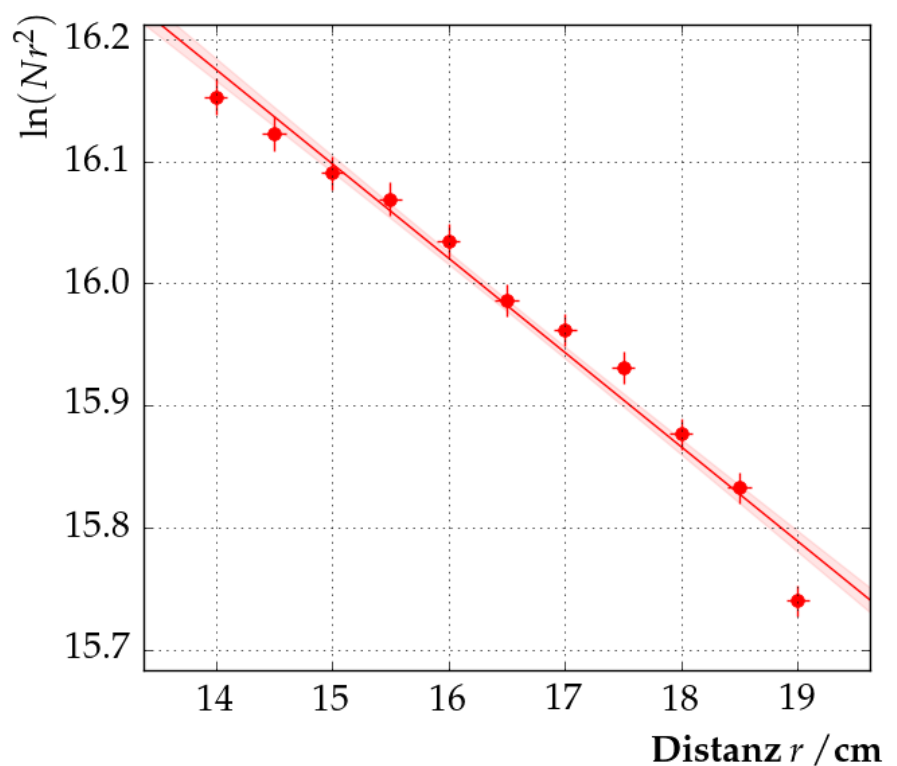
\includegraphics[scale=0.5]{./fig/plot1.png}
  \caption{Lineare Regression zur Bestimmung der Relaxationslänge (ohne Cd-Kugelschale)}
  \label{fig:plot1}
\end{figure}

\begin{figure}[tb]
  \centering
  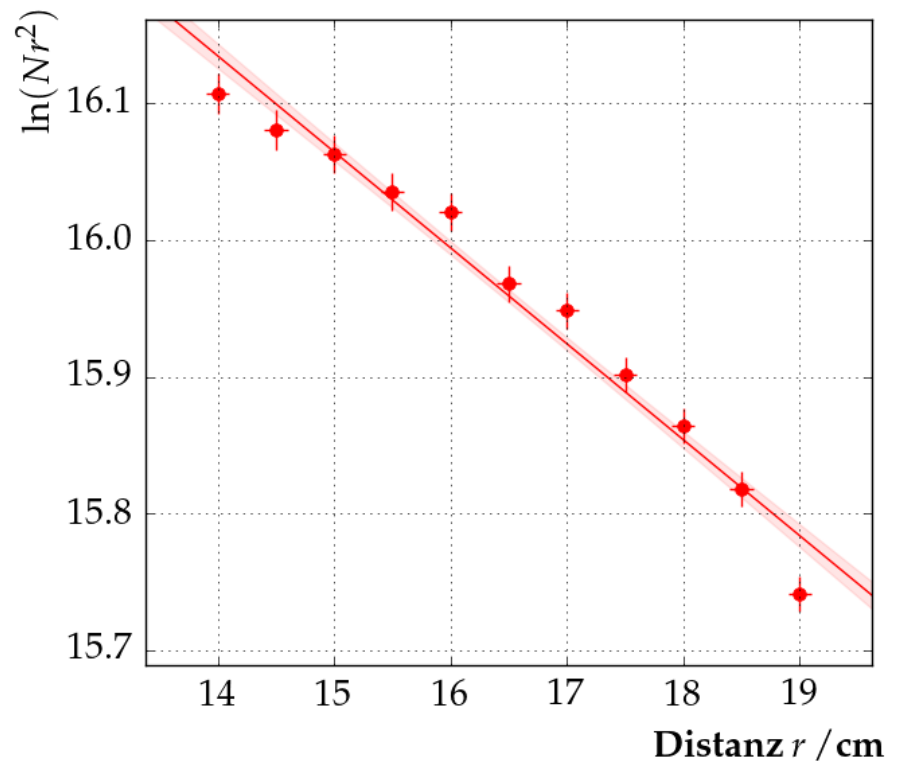
\includegraphics[scale=0.5]{./fig/plot2.png}
  \caption{Lineare Regression zur Bestimmung der Relaxationslänge (mit Cd-Kugelschale)}
  \label{fig:plot2}
\end{figure}

\section{Bestimmung der Diffusionslänge}

Der Fluss der thermischen Neutronen ist proportional zur Differenz aus der Anzahl der Neutronen ohne Abschirmung $N_{1}$ und der Anzahl der Neutronen mit Abschirmung $N_{2}$. Die Unsicherheit ist jeweils durch $\Delta N=\sqrt{N}$ gegeben.
Da die Unsicherheiten auf die beiden Messwerte korreliert sind, ergibt sich per Größtfehlerabschätzung
\begin{equation}
 \Delta N_{d} = \frac{\sqrt{N_{1}}+\sqrt{N_{2}}}{N_{1}-N_{2}},
\end{equation}
mit $N_{d}=N_{1}-N_{2}$.
Insgesamt ergibt sich für die Unsicherheit auf die Größe $y=\ln(N_{d}r)$
\begin{equation}
 \Delta y = \sqrt{\left(\frac{\Delta N_{d}}{N_{d}}\right)^{2}+\left(\frac{\Delta r}{r}\right)^{2}}.
\end{equation}

Der Messwert für $r=\SI{19}{\centi\metre}$ ist $N_{d}=-29<0$. Dies liegt jedoch innerhalb der Fehlergrenzen, denn $\Delta N_{d}=276$. Da der Logarithmus für negative Werte nicht definiert ist, wurde dieser Messwert nicht für die Regression verwendet.

Die lineare Regression der Form $y=ar+b$ wird mit ``kafe'' durchgeführt und ergibt (s. Abb. \ref{fig:plot3})
\begin{equation}
 a = \SI{-0,37\pm0,10}{\per\centi\metre}.
\end{equation}
Daraus folgt für die Diffusionslänge
\begin{equation}
 L = -\frac{1}{a} = \SI{2,7\pm0,7}{\centi\metre}.
\end{equation}
Der Literaturwert für $L$ liegt zwischen $\SI{2,85}{\centi\metre}$ und $\SI{3,6}{\centi\metre}$ \cite{DeJuren}. Der hier gemessene Wert liegt im Rahmen der Messunsicherheit in diesem Bereich.

\begin{figure}[tb]
  \centering
  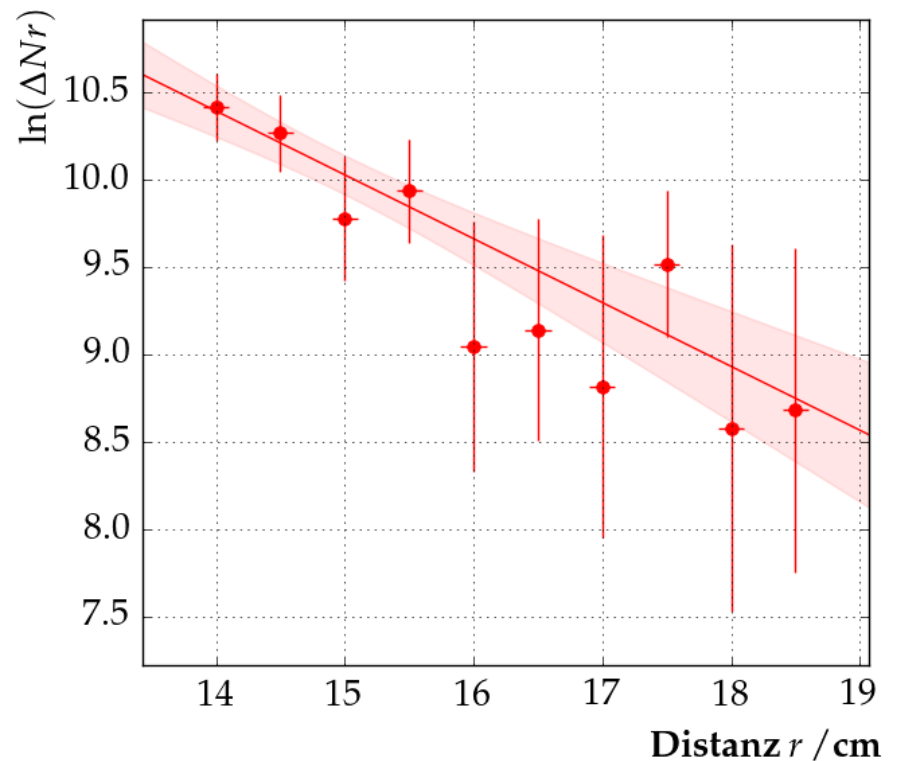
\includegraphics[scale=0.5]{./fig/plot3.png}
  \caption{Lineare Regression zur Bestimmung der Diffusionslänge}
  \label{fig:plot3}
\end{figure}

